\documentclass[11pt]{article}
\usepackage{amsmath,amssymb}
\usepackage{tikz}
\usetikzlibrary{arrows.meta,positioning,calc}
\usepackage[utf8]{inputenc}
\usepackage{hyperref}

% A documentation page about a converter is written with the converter. Everything
% below is ordinary LaTeX: the maths is maths, the figures are TikZ, the code is
% verbatim, and the tables are tables. If this page needs anything that is not in
% the source of a paper, the paper would need it too.
\title{Documentation}
\author{by leoldev}
\date{}

\begin{document}
\maketitle

\section{The command}

To use λtex2web, specify an input and an output. For example:

\begin{verbatim}
latex2web paper.tex site/
latex2web chapters/ site/                 // directory input
latex2web paper.tex --theme docs
latex2web paper.tex site/ my.config.json
\end{verbatim}

In essence, \texttt{λtex2web input output config}.

\subsection{Options}

\begin{tabular}{@{}ll@{}}
\texttt{-t, --theme} & \texttt{paper}, \texttt{slides} \\
\texttt{-p, --palette} & \texttt{warm-paper}, \texttt{catppuccin-frappe},
  \texttt{catppuccin-mocha}, \texttt{catppuccin-macchiato},
  \texttt{catppuccin-latte}, \texttt{warm-paper-dark} \\
\texttt{--tokens} & one or more colour tokens, as JSON, on the command line \\
\texttt{--css} & an extra stylesheet, appended after the layout's own \\
\texttt{--template} & replace the HTML shell entirely \\
\texttt{-F, --single-file} & inline the CSS, the maths and the fonts into one file \\
\texttt{--figures} & compile TikZ with a real engine when one is installed \\
\texttt{-I, --include-dir} & an extra search path for \texttt{\textbackslash input} \\
\texttt{--base} & a URL prefix for links when serving from a subdirectory \\
\texttt{-w, --watch} & rebuild when a source file changes \\
\end{tabular}

Flag has priority over configuration file, which has priority over the default.

\subsection{Single-file}

\texttt{--single-file} writes a \texttt{.html} including stylesheet, math
typesetting and the fonts to one file. Try:

\begin{verbatim}
latex2web paper.tex paper.html --single-file
\end{verbatim}

\section{Maths}

Maths is rendered, not imaged. \texttt{multiline}, \texttt{flalign},
\texttt{alignat}, \texttt{gather}, \texttt{equation}, \texttt{align},
\texttt{cases}, \texttt{array} and \texttt{pmatrix} all typeset:

\begin{equation}\label{eq:entropy}
  \mathcal{F}(g) = \int_M \bigl(R + |\nabla f|^2\bigr)\,e^{-f}\,dV.
\end{equation}

Cross-references resolve, so \eqref{eq:entropy} works. With
\verb|\numberwithin{equation}{section}| in the source, equations number inside
their section -- $(2.1)$, $(3.1)$ -- rather than running on for the whole paper.

\subsection{What is not rendered}

An environment the converter does not know is kept as source and labelled, never
dropped. A figure that will not compile is shown as the code that would have
produced it, with the reason.

\section{Figures}

\subsection{Graphics}

An extension-less \texttt{\textbackslash includegraphics} resolves the way LaTeX
resolves it. Vector artwork is rasterised at build time, because a PDF inside an
\texttt{<img>} displays nothing, and \texttt{trim} is honoured while that happens.

\begin{verbatim}
\includegraphics[width=0.8\textwidth]{figures/pipeline}   % .pdf found on disk
\end{verbatim}

\subsection{TikZ}

TikZ is compiled against the source's own preamble, so a figure looks the way it
was drawn: its macros, its styles and its colour names all resolve.

\begin{verbatim}
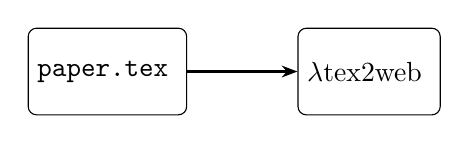
\begin{tikzpicture}[
  box/.style={draw, rounded corners=3pt, minimum height=1.1cm, align=center},
  flow/.style={-{Stealth[length=2mm]}, thick}
]
  \node[box] (a) { \texttt{paper.tex} };
  \node[box, right=1.4cm of a] (b) { $\lambda$tex2web };
  \draw[flow] (a) -- (b);
\end{tikzpicture}
\end{verbatim}

A build compiles it if it finds a TeX engine, and says so when it does not. With
no engine the drawing is shown as the source above, labelled as such.

\section{Layouts}

Five layouts, each usable with any palette.

\begin{description}
  \item[paper] Serif, print-inspired, generous measure, contents rail. For a
  paper.
  \item[notes] Sans-serif, wide measure, skimmable. For lecture notes.
  \item[slides] Scroll-snap deck. Sections become dividers, \texttt{beamer} frames
    become slides.
  \item[docs] Sections as cards, no rail. For a documentation page.
  \item[landing] A front page: the name set low, example buttons, a contents
    rail below the hero.
\end{description}

\section{Decks}

A \texttt{beamer} \texttt{frame} becomes a section, numbered the way beamer numbers
it. Each slide is labelled \texttt{Slide N of M} in document order; a
\texttt{[plain]} frame is not counted, because an opening card or a closing
\emph{The End} carries no number in the published deck either. A
\texttt{\textbackslash sectiontitleframe} is counted, and renders as a real heading.

Overlays are flattened. There is no presenter on a web page to reveal them.

\subsection{References to a sibling deck}

\texttt{\textbackslash dlcref} is Fleuret's cross-reference to another lecture in
the same course. It reads a \texttt{.dlcref} file that the other lecture writes,
so a deck on its own has nothing to resolve against. Supply the map instead:

\begin{verbatim}
{ "xrefs": { "einstein-summations": "1.5. ``High dimension tensors''" } }
\end{verbatim}
A key with no entry prints nothing and is reported. Printing the macro's
argument at the reader is what a broken cross-reference looks like.

\section{Palettes and tokens}

A palette is colour and type; a layout is structure. Six palettes ship, each
with a light and a dark half, so a page follows the reader's system. There is no
toggle
in the chrome.

\begin{verbatim}
--palette catppuccin-mocha
--tokens '{"accent":"#2f5fd0","accent-soft":"#e8effc"}'
\end{verbatim}

Colour and font tokens come from the palette: \texttt{bg}, \texttt{bg-raised},
\texttt{bg-sunken}, \texttt{bg-tint}, \texttt{ink}, \texttt{ink-soft},
\texttt{ink-faint}, \texttt{line}, \texttt{line-soft}, \texttt{accent},
\texttt{accent-soft}, \texttt{accent-ink}, \texttt{accent-2}, \texttt{mark},
\texttt{shadow}, the six \texttt{emph-*} colours, the \texttt{tok-*} colours used
by code, and the \texttt{serif}, \texttt{sans} and \texttt{mono} stacks.

Structural tokens come from the layout: \texttt{measure}, \texttt{rail},
\texttt{gutter}, \texttt{masthead-h} and the type scale.

\subsection{What is measured, and what is yours}

A palette states a ground and a character. The ramps around it are derived and
then
checked, not chosen by eye: text levels are ordered by contrast against the
ground, a card is lighter than the page in both modes, and every level clears
WCAG AA on
every surface it lands on. That is why a dark flavour's \texttt{bg-raised} is
not
its own \texttt{mantle} -- Catppuccin's mantle is darker than its base, which
made a card a hole in the page.

A token you pass yourself is never second-guessed. The repair runs over the
palette first, so \texttt{\{"accent": "\#e11"\}} is the red you asked for.

\section{The configuration file}

JSON, or a module exporting an object or a function. Found by walking up from
the working directory; \texttt{extends} names a preset path or package.

\begin{verbatim}
{
  "theme": "docs",
  "palette": { "light": "warm-paper", "dark": "catppuccin-mocha" },
  "tokens": { "accent": "#2f5fd0", "measure": "46rem" },
  "motion": "on",
  "notice": "A note about this document, shown above it.",
  "hero": "front-matter",
  "wordmarkHero": true,
  "home": "./",
  "github": "owner/repo",
  "nav": [
    { "label": "Examples", "items": [
      { "label": "Math", "href": "site/src.html" }
    ]},
    { "label": "Docs", "href": "./" }
  ],
  "footer": true,
  "footerTagline": "One command, one folder, no server.",
  "figures": { "delegate": true },
  "toc": true,
  "assets": { "dir": "assets" }
}
\end{verbatim}

\subsection{The same file as a module}

A module may export a function, which is how a build generates its configuration
instead of repeating it. A preset is a module too, and a file that extends one
is handed the preset's result to change.

\begin{verbatim}
// latex2web.config.mjs
export default {
  theme: 'docs',
  palette: { light: 'warm-paper', dark: 'catppuccin-mocha' },
  extends: './docs.preset.mjs',
  tokens: { measure: '46rem', accent: '#2f5fd0' },
  motion: 'on',
  github: 'owner/repo',
};
\end{verbatim}

\subsection{Keys}

\begin{description}
  \item[theme] the layout name.
  \item[palette] a name, or \texttt{\{light, dark\}} for a pair.
  \item[tokens] colour, type and metric overrides, merged over the layout's.
  \item[css] extra stylesheets, appended after the layout's own -- the supported
    way to restyle without forking a theme.
  \item[template] a path replacing the HTML shell. The shell is a template, so
    the whole page is replaceable rather than only decorated.
  \item[nav] the masthead menu. An entry with \texttt{items} is a dropdown. Left
    unset, a multi-page build links its own documents instead.
  \item[footer] \texttt{false} for a line of small print instead of the site
    footer, which is what a lone converted document wants.
  \item[hero] \texttt{"front-matter"} lifts the title, the author and the first
paragraph into the hero, so the contents starts level with the first section.
  \item[wordmarkHero] draw the mark as the title instead of setting the title
    as a heading.
  \item[notice] an editorial note above the content, for when a conversion had
    to change something.
  \item[xrefs] where \texttt{\textbackslash dlcref} resolves to, as a map from key
    to the text to print. See \emph{References to a sibling deck}.
  \item[motion] \texttt{"on"} or \texttt{"off"}. \texttt{"auto"} is not an alias
    for \texttt{"on"}.
  \item[figures] \texttt{\{delegate: false\}} stops the build shelling out to a TeX
    engine, for a build that must not reach the network or that wants the same
    bytes on a machine with TeX and one without. On by default.
  \item[head], \item[scripts] extra markup, or functions returning it.
\end{description}

An unknown key is reported rather than ignored, because a typo is silent
otherwise and the symptom is a setting that does not apply.

\section{What a conversion is not}

The source that was written is the source that is typeset. Nothing is rasterised
from a PDF of the document, because a PDF has already thrown away the structure
that makes a page worth reading: the headings are not headings, the references
are not links, the equations are pictures of equations.

So a converted paper is a conversion, not a transcription, and no claim is made
over the work itself. Where something had to change to get a page out at all,
\texttt{notice} is how that gets said on the page.

\section{Getting a page out of a real paper}

\begin{enumerate}
  \item Give it the source: \texttt{latex2web paper.tex site/}, then open
    \texttt{site/paper.html}.
  \item Pick a layout for what it is. A paper is \texttt{paper}, a deck is
    \texttt{slides}, notes are \texttt{notes}.
  \item A figure that comes out as source means no TeX engine was found to
    compile it. Installing one is all it takes.
  \item If a section came out wrong, check whether the source stars it.
    \texttt{\textbackslash section*} is unnumbered, and numbering it shifts every
    equation after it.
  \item If something is missing, say so on the page with \texttt{notice} rather
    than leaving the reader to find the gap.
\end{enumerate}

\end{document}


